\chapter{Studi Literatur}
\label{chapter:studi-literatur}

Bab ini akan diisi oleh studi literatur yang terkait dengan topik persoalan pada tugas akhir untuk memberikan informasi mengenai dasar teori dan literatur yang digunakan. Bab ini diharapkan dapat membantu pembaca memiliki pengetahuan yang menyeluruh dan dasar yang cukup untuk mengerti penelitian ini.

\section{Blockchain}

\textit{Blockchain} adalah sekuens dari blok yang menyimpan daftar transaksi lengkap seperti \textit{public ledger} konvensional, dimana setiap \textit{ledger} disimpan pada \textit{node} yang tersebar seperti pada \textit{Distributed Ledger Technology} \parencite{zheng2018blockchain}. Setiap transaksi yang masuk ke dalam sebuah blok akan divalidasi sesuai dengan metrik yang digunakan oleh sistem \textit{blockchain}, dan blok yang memiliki daftar transaksi yang lengkap, ditambah \textit{timestamp} pembuatan blok, nilai \textit{hash} dari blok sebelumnya ("\textit{parent}"), dan sebuah \textit{nonce}, yang adalah sebuah angka acak yang digunakan untuk mekanisme verifikasi \textit{hash}. Konsep ini memastikan integritas dari \textit{blockchain} dimulai dari blok pertama ("\textit{genesis block}") sampai ke blok terakhir, yang terus ditambahkan, karena setiap perubahan data akan membuat nilai \textit{hash} dari sebuah blok berubah, yang harus dipropagasikan ke setiap blok setelahnya. Sebelum ditambahkan ke dalam \textit{blockchain}, setiap blok dan transaksi di dalamnya harus divalidasi oleh mayoritas \textit{node}, menggunakan sebuah mekanisme \textit{consensus} \parencite{nofer2017blockchain}. Mekanisme \textit{consensus} adalah proses dimana mayoritas dari \textit{network validator} menyetujui atau menolak sebuah \textit{state} dari \textit{ledger}. Proses \textit{consensus} mengikuti sebuah kumpulan aturan dan prosedur untuk mempertahankan himpunan fakta yang koheren diantara beberapa \textit{participating nodes}. Terdapat banyak mekanisme \textit{consensus} yang berbeda yang digunakan dalam \textit{blockchain network} yang berbeda. Dalam kasus \textit{Bitcoin}, \textit{ledger} yang dianggap \textit{ledger} yang \textit{valid} adalah \textit{ledger} dengan \textit{chain} terpanjang (\textit{longest chain}) \parencite{swanson2015consensus}.

\begin{figure}[ht]
	\centering
	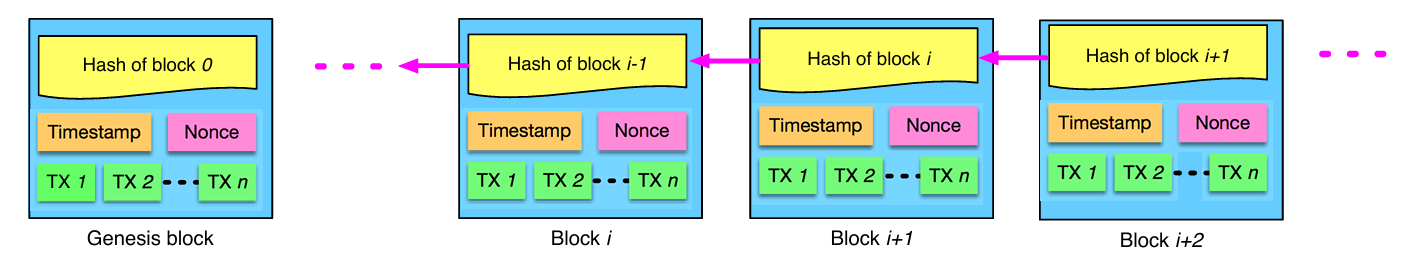
\includegraphics[width=1\textwidth]{resources/chapter-2/struktur-blockchain.png}
	\caption{Struktur blok di dalam \textit{blockchain} \parencite{zheng2018blockchain}}
	\label{image:struktur-blockchain}
\end{figure}

\break

Struktur dari sebuah blok terdiri dari \textit{block header} dan \textit{block body} seperti pada gambar \ref{image:struktur-blok}. Secara spesifik, \textit{block header} terdiri dari:

\begin{enumerate}
	\item \textit{Block Version}: mengindikasikan set dari aturan validasi yang diikuti.
	\item \textit{Parent Block Hash}: 256-bit \textit{hash} dari blok sebelumnya.
	\item \textit{Merkle Tree Root}: hasil \textit{hash} dari seluruh transaksi pada blok menggunakan mekanisme \textit{Merkle Tree}.
	\item \textit{Timestamp}: \textit{timestamp} saat ini dalam detik sejak 1970-01-01T00:00 UTC.
	\item \textit{nBits}: target \textit{hash} saat ini dalam format \textit{compact}.
	\item \textit{nonce}: \textit{number used only once}, sebuah angka yang digunakan untuk menambahkan tingkat keacakan dari nilai \textit{hash}.
\end{enumerate}

\begin{figure}
	\centering
	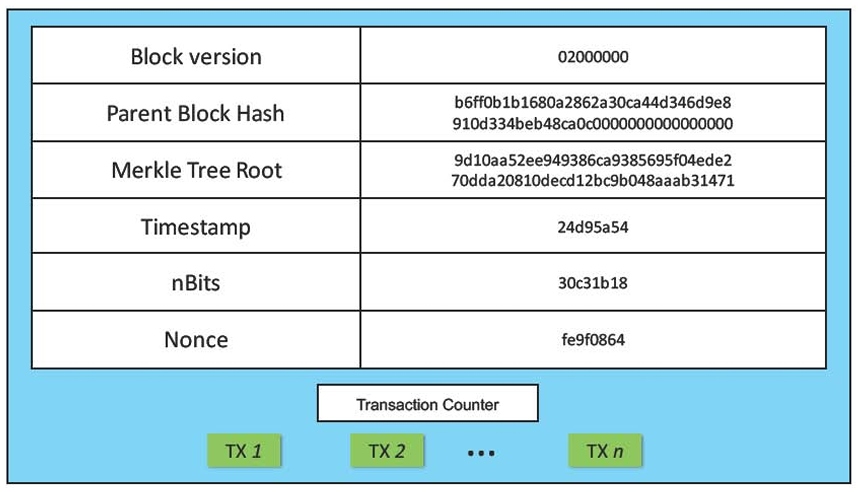
\includegraphics[width=0.7\textwidth]{resources/chapter-2/struktur-block.png}
	\caption{Struktur blok \parencite{zheng2018blockchain}}
	\label{image:struktur-blok}
\end{figure}



% \subsection{Contoh Subsubbab}
% \label{subsec:contoh-subsec}



% \subsubsection{Subsubsubbab}
% \blindtext

% \subsubsubsection{sub sub sub sub bab}
% \blindtext

% \begin{table}[h]
% 	\caption{Tabel random}
% 	\vspace{0.25cm}
% 	\begin{center}
% 		\begin{tabular}{|c|c|c|c|}
% 			\hline
% 			Title1 & Title2 & Title3 & Title4  \tabularnewline
% 			\hline
% 			1647   & 1.97   & 0.68   & 1.90 \tabularnewline
% 			2301   & 2.92   & 1.06   & 2.75 \tabularnewline
% 			2969   & 3.23   & 1.16   & 3.78 \tabularnewline
% 			3791   & 4.39   & 1.40   & 4.14 \tabularnewline
% 			4625   & 6.72   & 1.87   & 5.59 \tabularnewline
% 			\hline
% 		\end{tabular}
% 	\end{center}
% \end{table}

% Bab Studi Literatur digunakan untuk mendeskripsikan kajian literatur yang terkait dengan persoalan tugas akhir. Tujuan studi literatur adalah:

% \begin{enumerate}
% 	\item menunjukkan kepada pembaca adanya gap seperti pada rumusan masalah yang memang belum terselesaikan,
% 	\item memberikan pemahaman secukupnya kepada pembaca tentang teori atau pekerjaan terkait yang terkait langsung dengan penyelesaian persoalan, serta
% 	\item menyampaikan informasi apa saja yang sudah ditulis/dilaporkan oleh pihak lain (peneliti/Tugas Akhir/Tesis) tentang hasil penelitian/pekerjaan mereka yang sama atau mirip kaitannya dengan persoalan tugas akhir.
% \end{enumerate}

% Kita juga dapat memisah beberapa bagian latex untuk \textit{readability}. Kita dapat memasukan file latex lainnya dengan menggunakan fitur input. Berikut merupakan contoh ketika memasukan bagian contoh-subbab ke chapter-2


% \section{Menyisipkan Persamaan}

% Beberapa contoh menyisipkan persamaan.

% \subsection{Contoh Bikin Equation}
% \textbf{text tebal} dan ini \emph{miring}, bikin persamaan di baris yang sama, tinggal pake dolar2 $\Psi(\vec{r}_1,...,\vec{r}_N)$, sehingga persamaan Schr\"{o}dinger, terus, persamaan yang dinomeri kayak gini
% %ini contoh bikin persamaan, ..... :D
% \begin{equation}
% 	\left[ \sum_{i}^{N}-\frac{\hbar^2}{2m}\nabla_i^2 + \sum_{i}^{N}V(\vec{r}_i)+ \sum_{i<j}^{N}(\vec{r}_i,\vec{r}_j)\right]\Psi = E\Psi
% \end{equation}

% untuk $N$-elektron, dengan $\hat{H}$=Hamiltonian, $E$=Energi total, $\hat{T}$=Energi kinetik, $\hat{V}$=Energi potensial, dan $\hat{U}$=Interaksi ektron-elektron.

% \subsection{Bikin Matrix}
% Lalalallala.... bikin matrix sekarang, yang ini dikecilin, pake smaller
% 	{\smaller
% 		\begin{equation}
% 			\Psi({\bf r}_1, {\bf r}_2, \cdots {\bf r}_N) = \frac{1}{\sqrt{N!}}\left| \begin{array}{llcl}
% 				\phi_1({\bf r}_1)     & \phi_2({\bf r}_1)     & \cdots                & \phi_N({\bf r}_1)     \\
% 				\phi_1({\bf r}_2)     & \phi_2({\bf r}_2)     & \cdots                & \phi_N({\bf r}_2)     \\
% 				\phi_1({\bf r}_3)     & \phi_2({\bf r}_3)     & \cdots                & \phi_N({\bf r}_3)     \\
% 				\multicolumn{1}{c}{.} & \multicolumn{1}{c}{.} & \multicolumn{1}{c}{.} & \multicolumn{1}{c}{.} \\
% 				\multicolumn{1}{c}{.} & \multicolumn{1}{c}{.} & \multicolumn{1}{c}{.} & \multicolumn{1}{c}{.} \\
% 				\multicolumn{1}{c}{.} & \multicolumn{1}{c}{.} & \multicolumn{1}{c}{.} & \multicolumn{1}{c}{.} \\
% 				\phi_1({\bf r}_N)     & \phi_2({\bf r}_N)     & \cdots                & \phi_N({\bf r}_N)     \\
% 			\end{array} \right|
% 		\end{equation}
% 	}